% Material and Methods

\chapter{Material and Methods} \label{ch:mat_met}

This chapter offers more information about the materials and methods that were used in the implementation of the project.
The chapter provides better understanding of what \gls{lorawan} is and how it is used between the Lorix One gateway and \gls{lora} end devices.
ChirpStack server's features are explained more thoroughly to understand what the stack consists of. 
Lastly the Robot Framework and it's structure and used libraries are introduced.

\section{LoRaWAN}
\gls{lorawan} is A networking protocol that is based on \gls{lora} and maintained by the \gls{lora} Alliance\cite{lora_alliance:about_lorawan}.
It is specifically designed for low-power, battery-operated devices.
\gls{lorawan} facilitates long-range communication between devices, extending up to 15 kilometers.
This extended range proves invaluable in areas where devices are widely distributed, optimizing connectivity.
The long-range capability contributes to cost-effective deployments, enabling the coverage of extensive areas with a minimal number of gateways.

\gls{lorawan} signals exhibit excellent penetration capabilities, allowing them to traverse obstacles like walls and buildings, enhancing communication reliability.
Many \gls{iot} devices operate by transmitting small amounts of data at irregular intervals.
\gls{lorawan} emerges as an optimal solution for such occasional data transmissions with its capacity to transmit data at low rates.
This low data rate feature not only conserves energy in battery-operated devices but also ensures efficient use of network resources.

\gls{lorawan} networks boast scalability, accommodating a substantial number of devices.
This scalability proves vital for \gls{iot} implementations that collect data from a diverse array of sensors.
The adaptability to scale makes \gls{lorawan} well-suited for the dynamic and evolving nature of \gls{iot} deployments.

In this project, \gls{lorawan} technology plays a significant role in wireless connectivity.
The implementation involves LoRa end devices utilizing Over-The-Air Activation (OTAA) to establish connections with the LORIX One gateway.
The gateway functions as a bridge and connects the devices to the Chirpstack \gls{lorawan} network server stack.
At the beginning of each course, the teacher initiates the creation of a new application on the server and the addition of devices to that application.
This manual process, characterized by repetition, is targeted for automation to minimize the time commitment from educators.

The integration of \gls{lorawan} not only optimizes connectivity in widely distributed educational settings but also capitalizes on its long-range capabilities, low data rate support, and scalability, making it an efficient solution for \gls{iot} applications within the project.
\cite{lora-developer-portal:about}
\todo{CHECK  (\cite{}) https://lora-developers.semtech.com/documentation/tech-papers-and-guides/lora-and-lorawan/ FOR POSSIBLE IDEAS FOR FIGURES RELATED TO LORAWAN}

\section{LORIX One}
LORIX One is a \gls{lorawan} gateway developed by Wifx\cite{wifx:lorixone}.
The operating system that LORIX One uses is called LORIX OS and it is created particularly for LoRaWAN gateways.
In this project LORIX One is used as a connector to transmit data between the \gls{iot} devices and the Chirpstack Network Server bidirectionally.
The Lorix One also runs the ChirpStack Gateway \gls{os}.

\section{LoRA end device}
\todo{The \gls{lora} end device, that is referred throughout the thesis,  consists of three parts: Raspberry Pico Board, \gls{lora} radio module and MicroPython.
The device is implemented by a previous student in their thesis work\cite{theseus:gere-zoltan} and it is used by Metropolia University of Applied Sciences in some of the courses they offer for the students.}


\todo{The \gls{lora} end device is used in this project for testing purposes.
The device details are given to the excel file with some additional dummy ones.
The automation script provides a command to add the devices to the ChirpStack server and from the server it can be verified that when a device is powered, it is connected to the server and send data.
This data can be seen by opening the corresponding tab of the device details.
The school provided two Raspberry Pico boards and four \gls{lora} radio modules, as two modules can be attached to a a same board.
}

\section{Chirpstack}
ChirpStack is a LoRaWAN network server stack.
It is an open-source platform, which means the source code is freely accessible, enabling contributions and modifications from individuals. It allows anyone to engage in its development.
The course runs the ChirpStack V3 with the limitation, that the LORIX One's \gls{os} does not support the latest version (V4).
The ChirpStack server's stack consists of 5 sections: ChirpStack Gateway Bridge, ChirpStack Network server, ChirpStack Application Server, ChirpStack Concentratord, and ChirpStack Gateway \gls{os}.

\subsection{ChirpStack Gateway Bridge}
ChirpStack Gateway Bridge enables communication between the ChirpStack Network Server and \gls{lorawan} gateways.
The gateway that is used in this project is the LORIX One.
The \gls{lora} devices send \gls{lorawan} packets to the gateway, which forwards them to the ChirpStack Network Server using the \gls{lora} Packet Forwarder.
The Chirpstack Gateway Bridge is given with 3 Packet Forwarder backends: ChirpStack Concentratord, Semtech UDP Packet Forwarder, and Basic Station Packet Forwarder.
These backends convert protocols into a common data format for the server.
Additionally the Gateway Bridge provides 3 integrations for \gls{mqtt} protocols: a generic \gls{mqtt} broker, that can be used as a central hub for handling the \gls{mqtt} communication in a single network; the GCP Cloud IoT Core MQTT Bridge; and Azure IoT Hub MQTT Bridge.
These \gls{mqtt} bridges enable communication to transmit messages and data between separate \gls{mqtt} networks or brokers alongside with other systems and platforms such as the \gls{lora} devices that are connected to the ChirpStack Network Server.
\cite{chirpstack:gateway_bridge}

\subsection{ChirpStack Network server}
ChirpStack Network Server receives frames from the LORIX One gateway and removes any dublicates before processing them.
The Network server handles the authentication, \gls{lorawan} \gls{mac}-layer operations, together with the \gls{mac}-commands, communication with the ChirpStack Application server and scheduling of the downlink frames sent to the \gls{lora} devices.
\cite{chirpstack:network_server}

\subsection{ChirpStack Application Server}

ChirpStack Application Server handles the join-requests and the process of handling and encrypting application payloads.
It provides a web-interface and for connection with external services a \gls{grpc} and \gls{rest}ful \gls{api}.
The web-interface and \gls{api} provide thev ability to manage users, organizations, applications and devices.
The data from \gls{lora} devices can be sent and/or received over both \gls{mqtt}, and \gls{http} protocols, and by being  written directly into Influx\gls{db} system.
The ChirpStack Application Server provides a feature that allows to test gateway network coverage by pinging, if the network contains multiple gateways.
It also offers live possibilities for frame- and event-logging.
\cite{chirpstack:application_server}

\subsection{ChirpStack Concentratord}
Chirpstack Concentratord is a \gls{lora}(WAN) concentrator daemon and is used by one or multiple application to collaborate with the gateway equipment by using an \gls{api} that is based to a universal messaging library called ZeroMQ.
The source code is open-source, as the other components of the Chirpstack server stack.
Chirpstack Concentratord handles the hardware specifics by applying and abstracting them through the \gls{api}.
This allows the packet forwarding application to be divided from the gateway hardware.
\cite{chirpstack:concentratord}

\subsection{ChirpStack Gateway OS}
The ChirpStack Gateway \gls{os} is based on Linux and can be run on numerous models of different \gls{lora} gateways.
In this implementation the used gateway is Lorix One.
The ChirpStack gateway \gls{os} aims to ease the setup of the gateway by providing preinstallations to reduce the amount of steps it would require without the \gls{os}.
There are two different types of images the user can select from, the chirpstack-gateway-os-base and chirpstack-gateway-os-full.
This project uses the full version, which differs from the base one by providing the full running enviroments of the ChirpStack Network and Application servers, which are not include in the base image.
The \gls{os} can be accessed over \gls{ssh} by using any \gls{cli}.
Figure~\ref{fig:ChirpStack_gateway_os}
\cite{chirpstack:gateway_os}

\begin{figure}[ht]
  \centering
  {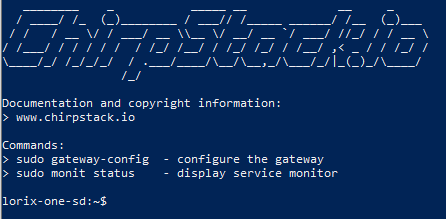
\includegraphics[width=\textwidth]{illustration/chirpstack_io_main_screen.PNG}}
  \caption{interface layout of ChirpStack Gateway OS full, when the user has logged in}
  \label{fig:ChirpStack_gateway_os}
\end{figure}

\section{Robot Framework}
Robot Framework is an open-source framework supported by Robot Framework Foundation and can be used for test automation and \gls{rpa}.
Robot Framework uses keywords that are in a human-readable format making its syntax easily accessible for technical and non-technical users.

The framework supports both data-driven and keyword-driven approaches for the implementations.
In data-driven approach the logic is separated from the data which allows to use the logic easily with multiple different inputs or data sets and keyword-driven approach focuses on creating keywords that give summary of the actions that the robot performs and which makes the maintainability, and readability more straightforward.

A Robot framework file's structure can contain 6 sections for the data: settings, variables, test cases, tasks, keywords and comments.
The sections are recognized by their header row that has a *** Settings *** format, which header is case-insensitive. The header can be surrounded with spaces but it is not necessary and the asterisk characters amount can also be different, but the minimum requirement is to have at least one asterisk in the beginning.
The headers can also contain other data besides the section header, but that data needs to be separated with the data format dependent separator.
That kind of extra headers are usually used for documenting.

Robot Framework contains standard libraries from which BuiltIn is the most used one and imported automatically.
The features can be extended by libraries that can be implemented in multiple different programming languages.

The following sections will provide understanding of what test suites and libraries are, and and how they can be used in the implementation of this project.

\subsection{Test suites}
A test case file that contains the automation tasks creates a test suite. Usually a test suite consists of ten or fewer tasks and the directory can have multiple test suites.
Automation of different processes can include similar pre-steps or afterwork that needs to be done every time a test suite is executed.
To make things more efficient a user can create Suite setup and teardown keywords that assist by doing the repeatedly needed steps.
These keywords have also the ability to accept arguments as needed.
Suite setup and teardown are declared in the suite initialization file.

A Suite setup is a keyword that is executed before any tasks are run.
If the setup fails, all the test suites that utilize it are directly assigned to fail status without being executed.
Suite setup offers possibilities to check preconditions that must be fulfilled before the automation tasks are being performed.

Similarly to a Suite setup, a Suite teardown is performed after the automation tasks are executed.
It is usually performed to clean up, and with a difference to a suite, if the suite setup fails the teardown is still being executed.
If the suite teardown fails, the test suites are marked as fail status regardless of their original status after execution.
\cite{robotFrameworkUserGuide:suiteSetupAndTeardown}

\subsection{Standard Library}
As mentioned in the beginning of this section, Robot Framework contains Standard Library that consist of ten libraries that can be imported to the projects with the exception of BuiltIn library that is imported by default.
These libraries include a wide spectrum of the most common tasks and verifications related to things such as date and time manipulations, collection handling, user inputs, operation system related tasks, process management and many others.
This project utilizes two of those libraries, the BuiltIn library and the Dialogs library.
Further information about them is explained in the next subsections.
\cite{robotFramework:standardLibrary}

\subsubsection{BuiltIn}
As mentioned previously BuiltIn is the only Standard Library in Robot Framework that is imported automatically.
It provides keywords that are the most generic ones and therefore needed often.
\cite{robotFramework:builtinLibrary}
\subsubsection{Dialogs}
Dialogs is part of the Standard Library and provides keywords to interact with the user. The keywords can be used to things such as to take user input or pause the execution until the user 
\cite{robotFramework:dialogsLibrary}

\subsubsection{Collections Library}
Collections library is part of Robot Framework's Standard Library.
The Collections library consists of keywords that can handle Python list and dictionaries.
The keywords can for example add or remove things from a list or dictionary, or search if a value is found from a list or dictionary.

\subsection{Browser Library}
Browser library is a Robot Framework library that delivers keywords for browser automation.
It uses Playwright framework to automate Chromium, Firefox and webkit.
The library offers a wide range of keywords, including getters for fetching information from various elements, classes, texts, and \gls{url}s.
Additionally, it includes keywords for waiting until certain elements are loaded or become visible before proceeding with the execution of subsequent keywords
\cite{robotFramework:browserLibrary}

\subsection{\gls{rpa} Framework}
Robocorp sponsors a  project called \gls{rpa} Framework, which is a collection of tools and libraries that can be used for \gls{rpa}.
The libraries are released under an open-source license.
Both the libraries and tools can be used with Robot Framework or Python.
This project uses one of the libraries from the collection, the RPA.Excel.Files.
\subsubsection{RPA.Excel.Files}
Robot framework features a library called RPA.Excel.Files which provides a large variation of keywords used to read and write data to Excel files.
The library enables the use of those files without the necessity of opening the Excel application.
\cite{rpaFramework:excelFiles}

\clearpage %force the next chapter to start on a new page. Keep that as the last line of your chapter!
